\documentclass{ohm_project_description}
\usepackage[english]{babel}

\projecttitle{Drone Swarm Obstacle Avoidance – Collision-Free Navigation of Micro-Drones}
\projectauthor{Mobile Robotics Lab}
\projectdate{2026}

\begin{document}

\maketitle
\thispagestyle{fancy}

\vspace*{-2.5cm}
\begin{figure}[h!]
    \centering
    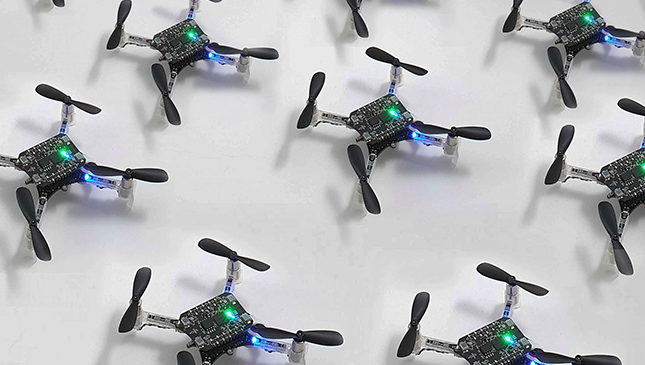
\includegraphics[height=4cm]{img/crazyflies.png}
\end{figure}

The Crazyflie micro-drones used at the AerodrOHM do not have dedicated onboard sensors for environmental perception. To enable safe interaction with people in the shared flight space, an external 3D camera is to be installed near the swarm. The goal is a system that reliably detects people in the shared flight space and controls the swarm so that drones automatically avoid and clear the way.

In the first step, the 3D camera is to be integrated into a ROS-based system architecture. The acquired point cloud data must be filtered, pre-processed, and transformed into an appropriate coordinate system. A central aspect is the classification of detected objects: the system must reliably distinguish between people and the drones themselves. Building on the person detection, a reactive swarm behaviour is to be developed that ensures safe coexistence in the shared space, including dynamic flight path adaptation and coordination of evasive manoeuvres. Practical testing takes place in the AerodrOHM flight space.

\section*{Work Packages}
\begin{itemize}[leftmargin=0.5cm]
    \setlength\itemsep{.1em}
    \item Integration and calibration of the external 3D camera
    \item Processing, filtering and transformation of point cloud data
    \item Development of a classification to distinguish between persons and drones
    \item Design and implementation of a reactive swarm behaviour with safety zones
    \item Test and evaluation in the flight space with real persons
\end{itemize}

\section*{Requirements}
\begin{itemize}[leftmargin=0.5cm]
    \setlength\itemsep{.1em}
    \item Programming skills (Python and/or C++)
    \item Ideally some experience with ROS
    \item Interest in sensor integration, point cloud processing and perception methods
\end{itemize}

\vspace{0.5cm}
This topic can be completed as a \textbf{project or master's thesis} subject to agreement.

\vfill
\textcolor{ohm_red}{\rule{\linewidth}{0.4mm}}
\textbf{\textcolor{ohm_red}{Mobile Robotics Lab}} \\
\begin{tabular}{@{}ll}
\textbf{Supervisor:} & Prof. Dr. Christian Pfitzner \\
\textbf{E-Mail:}     & \href{mailto:christian.pfitzner@th-nuernberg.de}{christian.pfitzner@th-nuernberg.de} \\
\end{tabular}

\end{document}
